\section{Method of alignment for the RICH optical system}
\label{sec:MirrorAlignmentMethod}

An iterative, data-driven method for finding appropriate software compensations for the mirror misalignments was developed in the HERAb experiment~\cite{Gorisek:1999td}. The approach presented here builds on that method and is developed further to address the more complex design of the \lhcb \rich system.\\

A misalignment in the \lhcb \rich optical system manifests itself as a displacement of the observed Cherenkov ring against the expected one \cite{Papanestis:2008zz, Baldini:2006ed} as can be seen in Figure \ref{fig:RICH_MisalignmentDiagrams}. This can also be viewed as a discrepancy between the actual center of the Cherenkov ring - e.g. the center of the Cherenkov ring observed on the detector plane -  and its expected position calculated from the projection of the track onto the detector plane using the orientation of the optical components given in the current \lhcb conditions database. 

\begin{figure}[hbt]
  \vspace{-0.5\baselineskip}
  \centering{
    \includegraphics[width=0.27\textwidth]{figs/Method/TiltedMirror}
    \hspace{0.07\textwidth}
    \includegraphics[width=0.61\textwidth]{figs/Method/ShiftedRing_andStripe}
  }
  \hspace{0.35\textwidth}(a)\hspace{0.52\textwidth}(b)\hspace{0.13\textwidth}
  \vspace{-0.5\baselineskip}
  \caption{
    (a) Schematic drawing of how a rotational misalignment of a \rich mirror (primary mirror in this example) causes shift of the actual centre $P'$ of the Cherenkov ring to $P$ on the photon detector plane. The projection of the track is drawn for explanatory purpose and represents the position of the expected centre of the Cherekov ring. (b) The expected Cherenkov angle \thetaC and the reconstructed Cherenkov angle $\theta$ are displayed. $P$ marks the position of the extrapolated track projection calculated without adjustments that would compensate any misalignments of the \rich mirrors, while $P'$ is the actual position of the centre of the ring and displaced by $\varTheta^z$ and $\varTheta^y$ with respect to $P'$ . Cherenkov angles $\theta$ are evaluated relative to $P$, and therefore, vary with $\phi$. The gray stripe represents area around the expected ring from which the photon hits are reconstructed. The width of this stripe is empirically chosen wide enough to cover the actual shifted (and somewhat smeared) ring of hits from a given track. Inevitably, the ``noise'' background photon hits in this area are also ``reconstructed''.}
  \label{fig:RICH_MisalignmentDiagrams}
  \vspace{-0.5\baselineskip}
\end{figure}

In order to observe and quantify the misalignment the quantity \deltatheta 
\begin{equation}
\delta\theta\left(\phi\right) = \theta\left(\phi\right) - \theta_{\mathrm{Ch}},
\end{equation}
-- where $\theta\left(\phi\right)$ is the the measured Cherenkov angle and $\theta_{\mathrm{Ch}}$ the expected Cherenkov angle -- is plotted against the azimuthal angle $\phi$ (see Figure \ref{fig:RICH_MisalignmentDiagrams}). For perfectly aligned mirrors \deltatheta is independent of $\phi$ but in case of a misalignment the distribution is approximately sinusoidal in $\phi$
\begin{equation}
  \label{eq:DeltaTheta_ps}
  \begin{aligned}
    \delta \theta_{p,s} (\phi) & \equiv   [\theta(\phi)-\theta_{\mathrm{Ch}} ]_{p,s}
                                 \approx  [\varTheta\cos(\phi-\varPhi)       ]_{p,s} \\
                               & =        [\varTheta\cos\varPhi\cos\phi
                                 +         \varTheta\sin\varPhi\sin\phi      ]_{p,s} \\
                               & =         \varTheta^z_{p,s}\cos\phi
                                 +         \varTheta^y_{p,s}\sin\phi                 \\
  \end{aligned}
\end{equation}
where the factors $\varTheta^y_{p,s}$ and $\varTheta^z_{p,s}$ represent the misalignments on the detector plane in $y$ and $z$ for a given mirror combination with primary mirror $p$ and secondary mirror $s$.\\
The misalignment factors $\varTheta^y_{p,s}$ and $\varTheta^z_{p,s}$ relate to the individual misalignments of the primary and secondary mirror via the \textit{magnification factors}
\begin{equation}
  \label{eq:theta0_y_z}
  \begin{aligned}
      A^y_{p,s}\alpha^y_p+B^y_{p,s}\beta^y_s
    + a^y_{p,s}\alpha^z_p+b^y_{p,s}\beta^z_s & = \varTheta^y_{p,s} \\
      A^z_{p,s}\alpha^z_p+B^z_{p,s}\beta^z_s
    + a^z_{p,s}\alpha^y_p+b^z_{p,s}\beta^y_s & = \varTheta^z_{p,s}
  \end{aligned}
\end{equation}
where $\alpha^y_p$, $\alpha^z_p$, $\beta^y_s$ and $\beta^z_s$ are the actual tilts of the primary and secondary mirrors around the $y$- and $z$-axis with respect to a given database. The magnification factors $A^y_{p,s}$, $B^y_{p,s}$, $a^y_{p,s}$ and $b^y_{p,s}$ ($A^z_{p,s}$, $B^z_{p,s}$, $a^z_{p,s}$ and $b^z_{p,s}$ for the $z$-axis) translate the effect of a tilt of the mirrors onto the detector plane (see Section \ref{subsec:Magnification}).\\
After all individual mirror tilts have been calculated a new database with the mirror orientations is created. It is useful to apply the alignment procedure iteratively to the same data sample, each time with the new database produced by the previous alignment. The alignment procedure is considered to have converged after no mirror has been found to have a misalignment greater than a chosen convergence criteria. \\
An overview of the entire alignment procedure can be seen in Figure \ref{fig:RICH_Procedure} while different details of the procedure are explained in the sections below.\\

\begin{figure}[h!]
  \centering{
    \includegraphics[width=0.7\textwidth]{figs/Method/procedure}
  }
  \vspace{-0.5\baselineskip}
  \caption{Overview of the entire alignment procedure. The alignment starts from a sample of events and usually from the mirror orientation given in the \lhcb conditions database. From there high energy tracks are reconstructed under the pion hypothesis (see Section \ref{subsec:TrackSelection}). Then the \deltatheta vs. $\phi$ histograms are filled for each mirror combination selected for the alignment procedure (see Section \ref{subsec:IndivMirrAlign}) and fitted to get the misalignments on the detector plane. With these the individual mirror misalignments are determined and a new database containing the corrected mirror orientations is created. If the convergence criteria is reached the alignment procedure is finished, if the criteria has not been reached the newly made database is used for the reconstruction of the same events and the entire procedure is repeated.}
  \label{fig:RICH_Procedure}
  \vspace{-0.5\baselineskip}
\end{figure}


\subsection{Track and photon selection}
\label{subsec:TrackSelection}
The events that the tracks and their photons are taken from are preselected. More information about the preselection and its implementation is given in Section \ref{sec:OnlineAlignmentFramework}.\\
In order to most accurately predict the Cherenkov angle for a given track some selection criteria are applied to the tracks themselves and to the photon candidates that make it into the \deltatheta vs. $\phi$ histograms.\\
High-momentum tracks are selected where the assumption can be made that the Cherenkov angle is saturated and therefore does not depend on the particle type any more. Figure \ref{fig:saturation} and Equation \ref{eq:DeltaTheta_ps} show the dependency of the Cherenkov angle of the momentum $p$ for different types of particles with mass $m$ in a radiator with refractive index $\eta$. 
\begin{equation}
  \label{eq:thetaC}
 \theta_{\mathrm{Ch}} = \arccos\left( \frac{1}{\eta} \sqrt{\left(\frac{m}{p}\right)^{2} + 1}  \right)
\end{equation}
In the case of high energy tracks all particles are assumed to have the the mass of a pion and the expected Cherenkov angle is calculated under that hypothesis.\\
\begin{figure}[htbp]
  \vspace{-0.5\baselineskip}
  \centering
  \includegraphics[width=0.75\textwidth]{figs/Method/ThetaVsMomentum_C4F10}
  \vspace{-0.5\baselineskip}
  \caption{
    Cherenkov angle \thetaC against track momentum, for tracks traversing the \richone gaseous radiator. Muons, pions, kaons and protons are visible. As the track momentum  increases, all particles tend towards the same \thetaC, known as the saturated Cherenkov angle.}
  \label{fig:saturation}
  \vspace{-0.5\baselineskip}
\end{figure}
The photon hits chosen to fill the \deltatheta vs. $\phi$ histograms are chosen from a ring-shaped area around the expected center of the Cherenkov ring (see Figure \ref{fig:RICH_MisalignmentDiagrams}). The ring's width is chosen to be big enough to cover the area of a shifted Cherenkov ring from a potentially misaligned mirror combination.\\
In the calculation of \deltatheta for the histograms the value for $\theta\left(\phi\right)$ is needed. This value is obtained by matching a photon hit on the detector plane to a track and calculating the Cherenkov angle. This requires an assumption about where along the track the Cherenkov photon was emitted. Since this is a intrinsically unknown quantity the assumption is made that the photon was emitted in the middle of the track. This introduces a source of noise from photons falsely associated with a given track. An analysis of MC events has shown~\cite{Gorisek:1999td} that it is possible to reduce this noise by only reconstructing \textit{unambiguous} photon hits. A photon hit is \textit{unambiguous} if it will be reflected by the same primary and secondary mirror independently of where along the particle track it was emitted. Therefore only unambiguous photon hits are chosen to be used in the alignment procedure in the \deltatheta vs. $\phi$ histograms.\\


\subsection{Method for fitting the \deltatheta vs. $\phi$ distributions}
\label{subsec:Fitting}

For every chosen combination of primary mirror $p$ and secondary mirror $s$, \deltatheta is plotted against $\phi$. Each of these two-dimensional distributions is divided into 20 bins in $\phi$. Inside each $\phi$ bin the \deltatheta distribution is fitted with a Gaussian plus a second order polynomial that represents the background photons. In accordance with Equation~\ref{eq:DeltaTheta_ps} the $\phi$ dependence of the position of the Gaussian peak for a given mirror combination $(p,s)$ is approximated by
\begin{equation}
  \label{eq:Delta_theta}
  \delta\theta_{p,s}(\phi) = \varTheta^z_{p,s}\cos\phi
                           + \varTheta^y_{p,s}\sin\phi.                         
\end{equation}
Equation~\ref{eq:Delta_theta} is used as a bond when fitting all the 20 slices jointly.\\
The fitting is done by means of the \root framework~\cite{Antcheva:2011zz}, in particular, using the \minuit minimization package. An example of a \deltatheta vs. $\phi$ histogram for a specific mirror combination in \richone, including the fitted sinusoidal of Equation \ref{eq:Delta_theta} is shown in Figure \ref{fig:Rich1Mirr0001dThetavphiRec}, before alignment and after the alignment.
\begin{figure}[htbp]
  \vspace{-0.5\baselineskip}
  \centering
  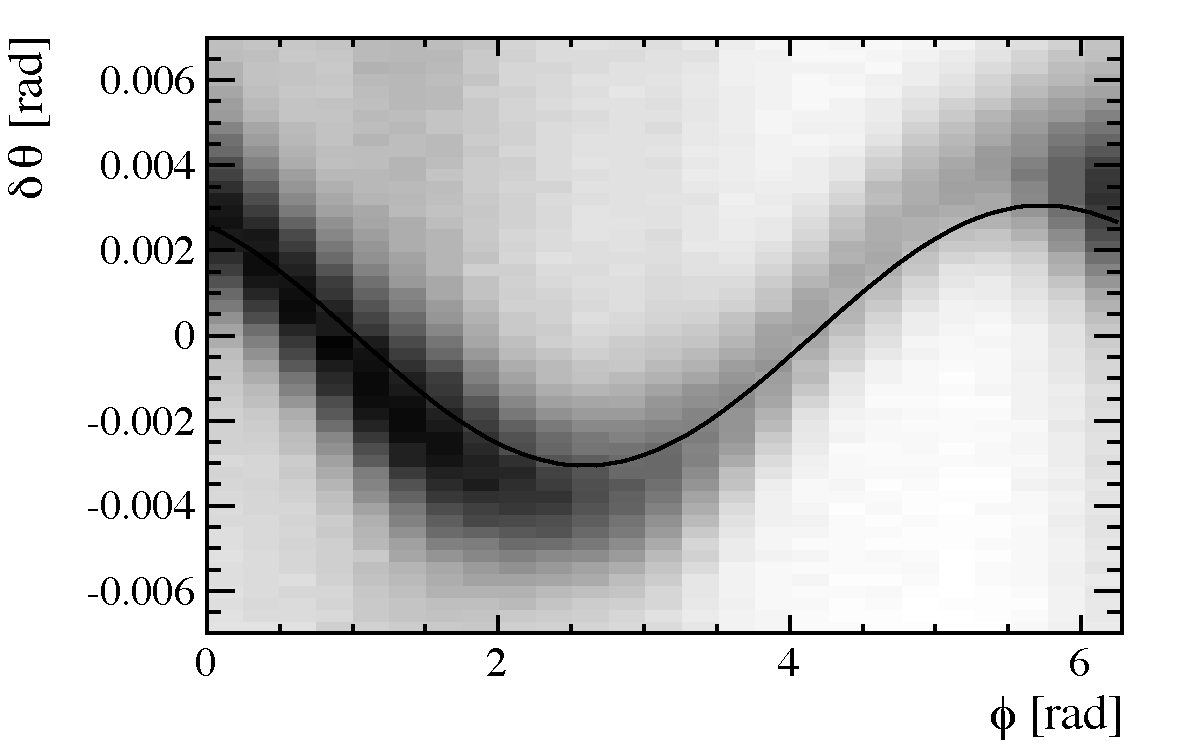
\includegraphics[width=.49\textwidth]
    {figs/Method/RICH1_ThetaVsPhiRec0001_misaligned.pdf}
  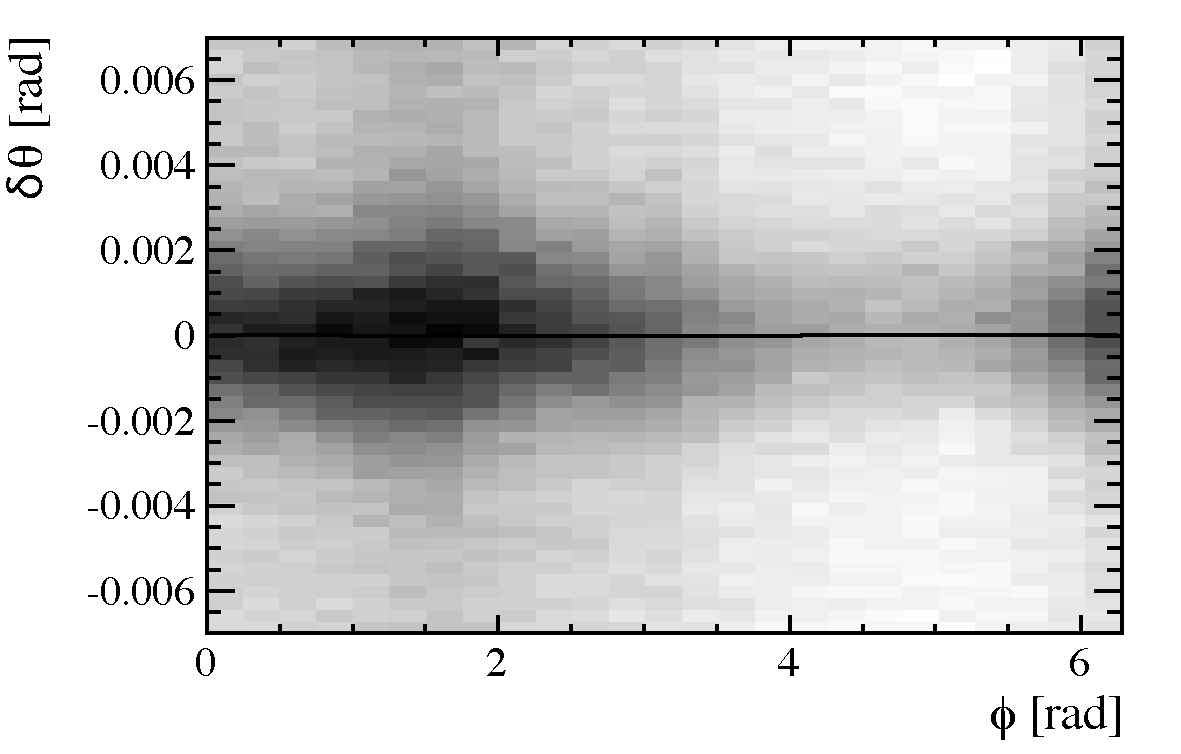
\includegraphics[width=.49\textwidth]
    {figs/Method/RICH1_ThetaVsPhiRec0001_aligned.pdf}
  \vspace{-1.0\baselineskip}
  \caption{
    \deltatheta against $\phi$ fitted slice-by-slice along $\phi$ with the function~\eqref{eq:Delta_theta} approximating the position of the Gaussian peaks on the $\phi\text{-}\delta\theta$~plane for the combination of primary mirror 0 and secondary mirror 1 of the \richone. The originally misaligned mirror combination is represented on the left while the right plot shows the same mirror combination after the alignment procedure.}
  \label{fig:Rich1Mirr0001dThetavphiRec}
  \vspace{-0.5\baselineskip}
\end{figure}


\subsection{Magnification factors}
\label{subsec:Magnification}
The magnification factors relate the tilts of the individual mirrors to the misalignment that can be observed in the detector plane. The effect of the magnification factors can be demonstrated in a simplified manner  by considering small rotations of primary and secondary mirrors around their $y$- axes. Those small rotations yield approximately the following displacement of the observable Cherenkov ring (as shown in~\fig{fig:RICH_MisalignmentDiagrams}):
\begin{equation}
l\,\varTheta^y \approx l_{\mathrm{pri}}2\,\alpha^y
                       - l_{\mathrm{sec}}2\, \beta^y,
\end{equation}
where $l$, $l_{\mathrm{pri}}$ and $l_{\mathrm{sec}}$ are lengths' of the paths of the photons to the photon detectors (from the emission point, from the primary mirror, and from the secondary mirror, respectively). Dividing this by the total photon path $l$ yields
\begin{equation}
\label{eq:magy}
  \varTheta^y  \approx \dfrac{2\,l_{\mathrm{pri}}}{l}\alpha^y
                     - \dfrac{2\,l_{\mathrm{sec}}}{l} \beta^y
               \approx                            A^y\alpha^y
                                                + B^y \beta^y
\end{equation}
where the factors in front of the actual mirror tilts $\alpha^y$ and $\beta^y$ are defined to be the magnification factors. The above equation is for illustrative purposes only and represents a simplified view because is doesn't take effects from rotations around the alternative (here $z$-) axis into account. The full expression used in the alignment procedure is shown in Equation \ref{eq:theta0_y_z}.\\
The magnification factors are determined using a data-driven method. Eight independent calibrational rotations (positive/negative rotations about the $y$- / $z$- axis for the primary and secondary mirrors) are introduced. Then the resulting misalignment on the detector plane is measured and used to solve Equation \ref{eq:magy} for the magnification factors. The final value of each magnification factor is arithmetical mean of the two corresponding values obtained with the calibrational rotations in opposite directions.\\
The size of each calibrational rotation for \richone is chosen to be $\pm0.7\mrad$ in order to sufficiently determine the magnification factors. This choice is motivated by the fact that the Cherenkov angle resolution for \richone is around $1.6\mrad$. Due to the smaller resolution of $0.7\mrad$ in \richtwo, the size of its calibrational rotations is chosen to be $\pm0.3\mrad$.\\


\subsection{Determining individual mirror misalignments}
\label{subsec:IndivMirrAlign}
The fits to the \deltatheta vs. $\phi$ distributions yield the misalignments in $y$ and $z$ on the detector plane for a given mirror combination. In order to determine the actual positioning of the mirrors for the \lhcb conditions database, the misalignments of the individual primary and and secondary mirrors are needed. This gives a system with more unknowns (individual mirror misalignments in $y$ and $z$) than equations. However, an optimal alignment can be achieved if each component of the optical system is properly aligned relative to all others. Therefore all mirrors only need to be aligned with respect to each other.\\


*** Needs to be written. ***

